\documentclass[12pt]{article}

\usepackage{complexity}
\usepackage{cmap}
\usepackage[T2A]{fontenc}
\usepackage[utf8]{inputenc}
\usepackage[russian]{babel}
\usepackage{graphicx}
\usepackage{amsthm,amsmath,amssymb}
\usepackage[russian,colorlinks=true,urlcolor=red,linkcolor=blue]{hyperref}
\usepackage{enumerate}
\usepackage{datetime}
\usepackage{minted}
\usepackage{fancyhdr}
\usepackage{lastpage}
\usepackage{color}
\usepackage{verbatim}
\usepackage{tikz}
\usepackage{epstopdf}
\usepackage{enumitem}
\usepackage{pdfpages}
\usepackage{array}

\def\THEME{Design document}

\begin{document}

\begin{center}
{\LARGE \bf \THEME}
\end{center}

\begin{center}
\vspace*{0.1cm}
{\Large \textit{\textbf{Общие сведения о системе}}}
\end{center}

\begin{center}
\vspace*{0.1cm}
{\large \textit{Описание}}
\end{center}

Игра жанра \texttt{Rogue-like}. Это консольная однопользовательская игра с сохранением. Основная цель~--- добраться до последнего уровня игры.

Главный персонаж~--- герой с исходными параметрами (здоровье, скорость, сила). В процессе игры пользователь управляет героем посредством клавиатуры. За одно нажатие совершается одно действие или перемещение на одну клетку карты.

В каждой клетке может находится препятствие, враг или предмет. При попытке переместиться в клетку с врагом происходит поочередная атака.
 
При перемещении в клетку с предметом предмет добавляется в инвентарь игрока. Игрок может использовать предметы из инвентаря и с их помощью улучшать параметры героя.

Каждый уровень генерируется случайным образом и состоит из карты с комнатами, соединенных проходами. Переход от одного уровня к другому осуществляется по специальному проходу.

Если у героя заканчивается здоровье, он умирает без возможности сохранения. Игра заканчивается и начать её можно только сначала.
 
\begin{center}
\vspace*{0.1cm}
{\large \textit{Функциональные требования}}
\end{center}

\begin{itemize}
\item Генерация уровней;
\item Наличие меню;
\item Возможность сохранения прогресса;
\item Возможность загрузки уровня;
\item Различные виды врагов и предметов;
\item Возможность улучшения характеристик героя;
\item Наличие инструкции к игре.
\end{itemize}

\begin{center}
\vspace*{0.1cm}
{\large \textit{Ограничения}}
\end{center}

\begin{itemize}
\item Пошаговость. За одну команду осуществляется один ход.
\item Наличие временного приоритета у героя и различных видов врагов при атаке.
\item Процедурная генерация. Процедурно генерируются уровни, враги и предметы.
\item Размер карты уровня не ограничивается пространством.
\item Графика реализована с помощью текстовых символов на экране.
\item Интерфейс и управление. 
\item Наличие набора свойств у героя, предметов, врагов и местности, которые влияют на владельца и его окружение.
\item Необратимая смерть героя. Игрок должен начинать игру с начала и не может загрузить последнее сохранение.
\end{itemize}

\begin{center}
\vspace*{0.1cm}
{\Large \textit{\textbf{Architectural drivers}}}
\end{center}

\begin{center}
\begin{tabular}{| c |p{10cm}|}
\hline
Расширяемость & Герою, врагам и предметам присваиваются различные типы параметров. Гибкая и расширяемая система настроек позволит не фиксировать изначально каждый тип отдельно и позволит добавлять новые параметры.\\
\hline
Переносимость & Возможность запуска с различных устройств без загрузки дополнительного программного обеспечения.\\
\hline
Производительность & Быстрое отображение команды пользователя. Среднее время отображение изменений на экран~--- 0,1 секунда.\\
\hline
Удобство использования & Интуитивная доступность и простота в управлении игрой, наличие инструкции.\\
\hline
Готовность & Осуществления процесса игры с минимальным набором исходных параметров.\\
\hline
\end{tabular}
\end{center}

\begin{center}
\vspace*{0.1cm}
{\Large \textit{\textbf{Роли и случаи использования}}}
\end{center}

\textbf{Основные действующие лица и их главные цели:}

\begin{itemize}
\item Пользователь. Осуществляет процесс игры с помощью команд.
\item Разработчики. Реализуют и сопровождают игру. 
\end{itemize}

\textbf{Описание типичного пользователя:}

\begin{itemize}
\item Пользователь является человеком возрастом от 10 и более лет, вне зависимости от пола, национальности и сферы деятельности. 
\item Для взаимодействия с игрой опыт не является обязательным. 
\item Основная идея использования игры пользователем~--- обеспечить досуг, без определенного ограничения по времени процесса игры.
\item Необходимо, чтобы основные ожидания пользователя от жанра оправдались. Обеспечить играбельность и доступность процесса.
\end{itemize}

\begin{center}
\vspace*{0.1cm}
{\Large \textit{\textbf{Композиция}}}

(\texttt{Game Components Diagram} в конце документа)
\end{center}

Внутри система устроена по принципу \texttt{Model-View-Controller}.

Команды пользователя обрабатывает \texttt{KeyboardHandler}, являющийся частью блока \texttt{Controller}. Результат \texttt{KeyboardHandler} превращается в высокоуровневую команду при помощи фабрики \texttt{CommandFactory} и передаётся в \texttt{Model}.

Вся логика игры реализована в блоке \texttt{Model}, где основным классом является \texttt{GameState}.

Результат выполнения команды на экран пользователю отображает класс \texttt{UI}, являющийся частью блока \texttt{View}.

\begin{center}
\vspace*{0.1cm}
{\Large \textit{\textbf{Логическая структура}}}

(\texttt{Game Class Diagram} в конце документа)
\end{center}

Система состоит из трёх крупных классов: \texttt{UI}, \texttt{Controller} и \texttt{Model}.

Главная функция \texttt{UI}~--- \texttt{print\_map}~--- печатает карту на экран пользователю.

Главная функция \texttt{Controller}~--- \texttt{run}~--- обрабатывает команду пользователя, трансформируя её в высокоуровненый класс \texttt{Command}, и передаёт её в \texttt{Model}.

Главная функция \texttt{Model}~--- \texttt{process\_command}~--- обрабатывает команду, изменяя состояние игры, и возвращает карту для отрисовки \texttt{UI}.

\begin{center}
\vspace*{0.1cm}
{\Large \textit{\textbf{Взаимодействия}}}

(\texttt{Game Sequence Diagram} в конце документа)
\end{center}

Команда пользователя обрабатывается \texttt{KeyboardHandler}, затем трансформируется \texttt{CommandFactory} в высокоуровневый класс. Результат передаётся в \texttt{Model}, который обрабатывает команду, изменяет состояние игры и возвращает карту \texttt{UI} для отрисовки пользователю.

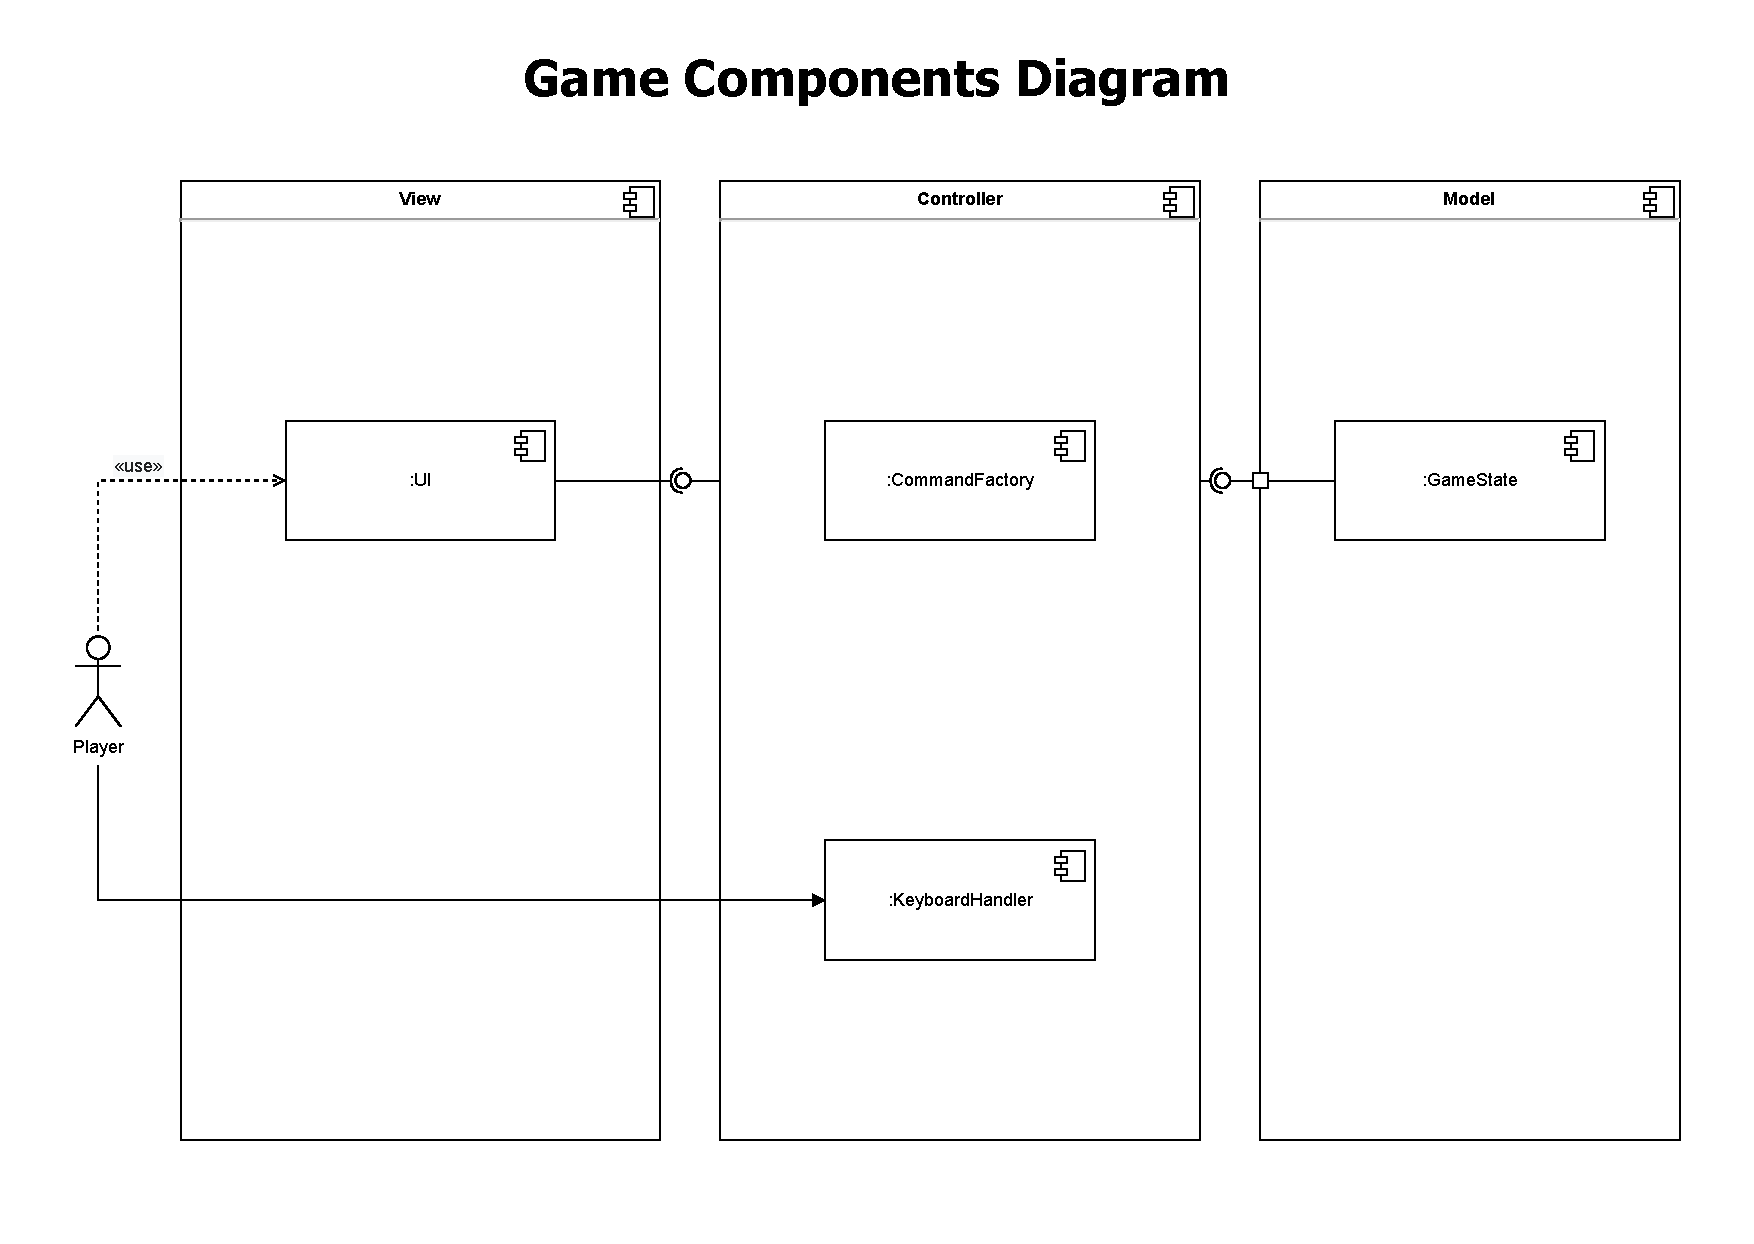
\includepdf{game_components_diagram.pdf}
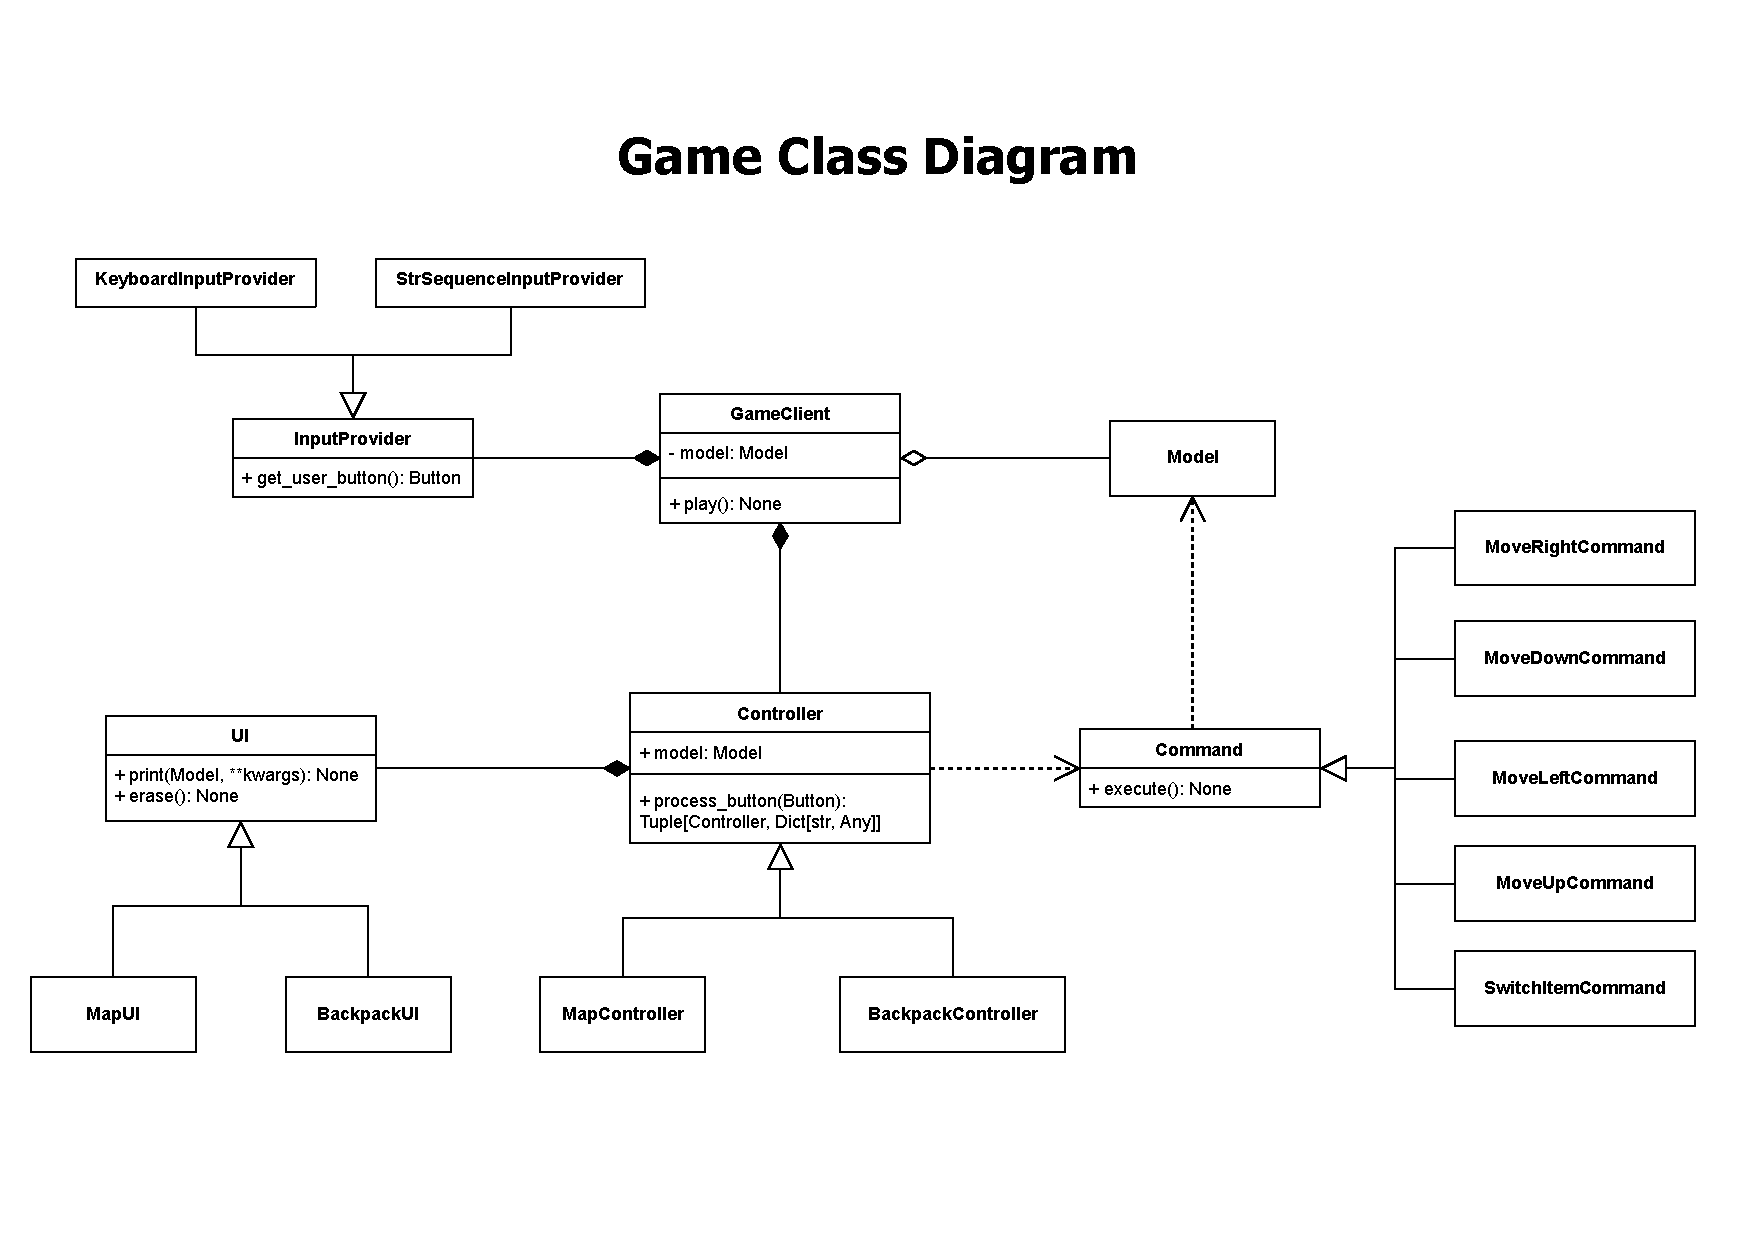
\includepdf{game_class_diagram.pdf}
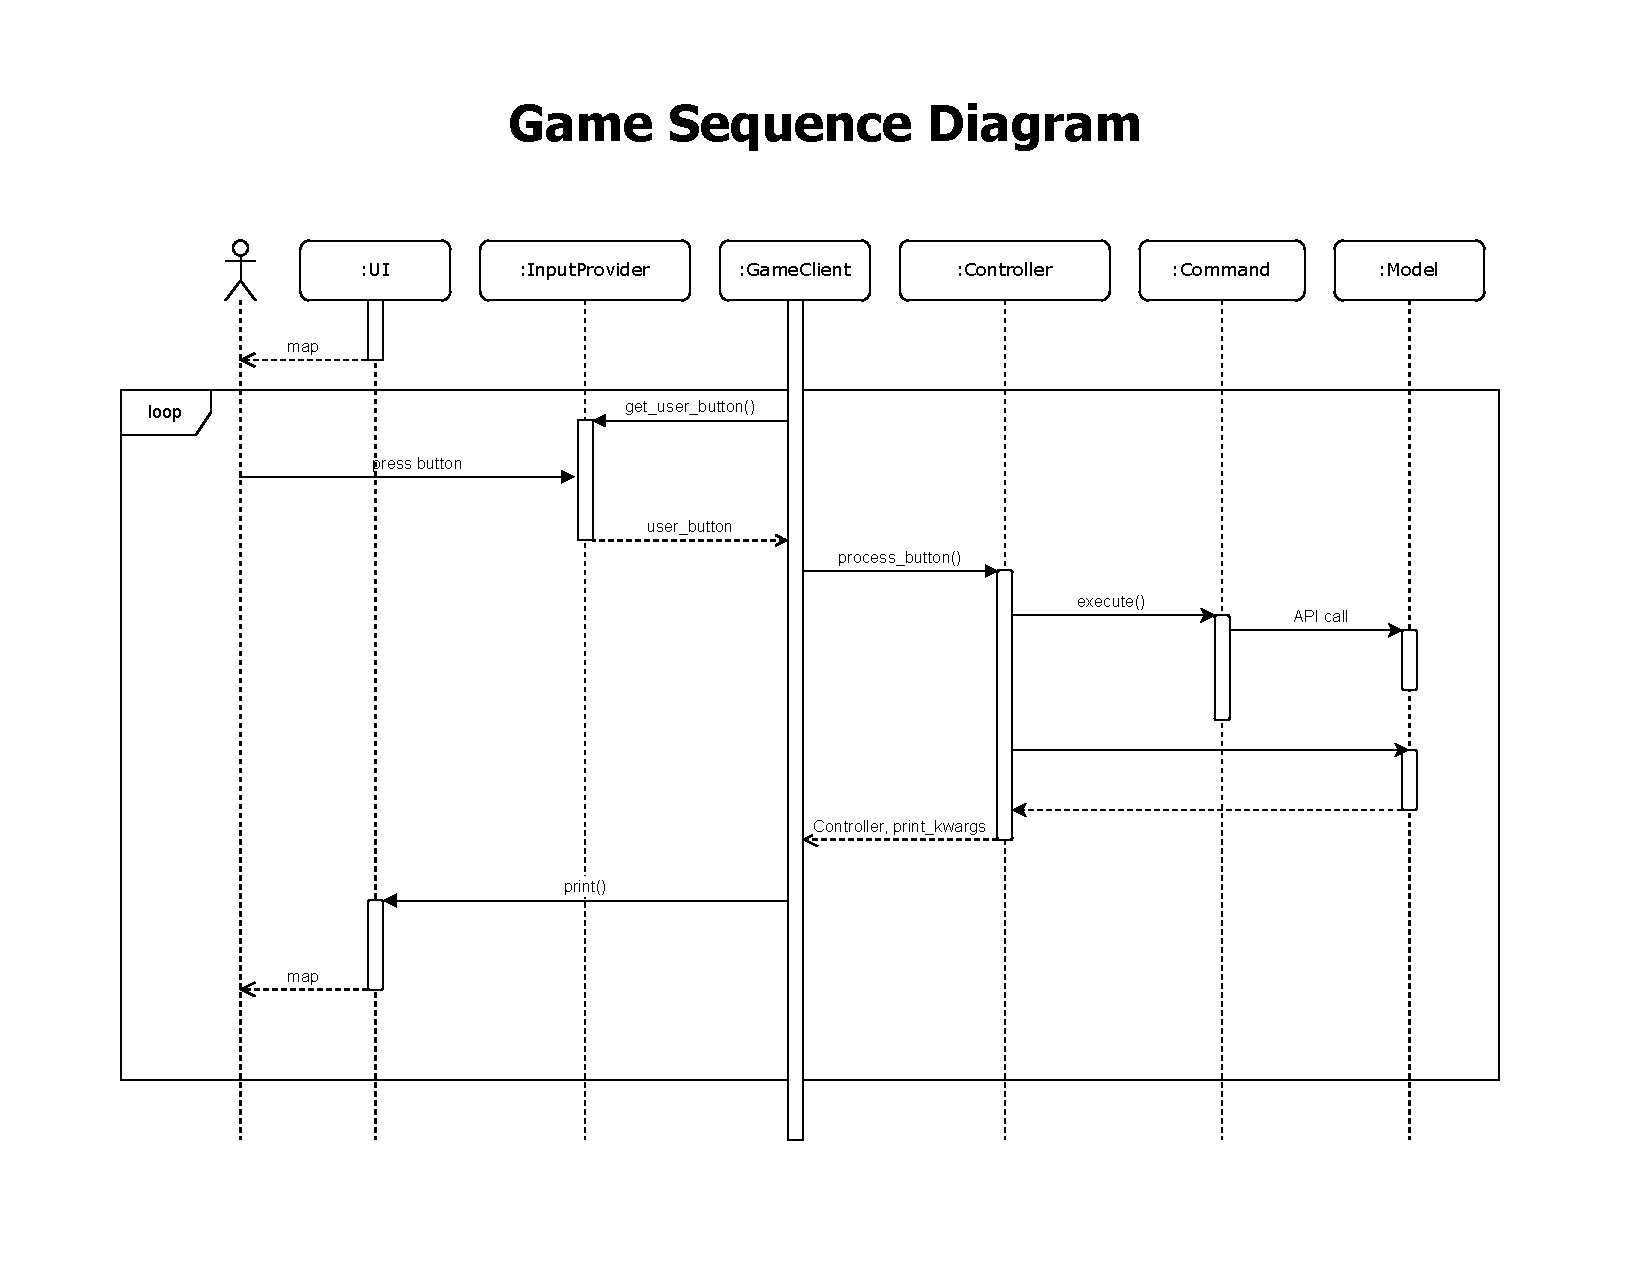
\includepdf{game_sequence_diagram.pdf}

\end{document}